\documentclass[letterpaper]{article}
% Set target color model to RGB
\usepackage[inner=2cm,outer=2cm,top=2cm,bottom=2cm]{geometry}
\usepackage{setspace}
\usepackage[rgb]{xcolor}
\usepackage{lmodern}
\usepackage{float}
\usepackage{verbatim}
\usepackage{caption}
\usepackage{subcaption}
\usepackage{amsgen,amsmath,amstext,amsbsy,amsopn,tikz,amssymb,tkz-linknodes}
\usepackage{fancyhdr}
\usepackage[colorlinks=true, urlcolor=blue,  linkcolor=blue, citecolor=blue]{hyperref}
\usepackage[colorinlistoftodos]{todonotes}
\usepackage{rotating}
\usepackage{listings}
\usepackage{minted}
\usemintedstyle{vs}
%\usetikzlibrary{through,backgrounds}
\hypersetup{%
pdfauthor={Ashudeep Singh},%
pdftitle={Homework},%
pdfkeywords={Tikz,latex,bootstrap,uncertaintes},%
pdfcreator={PDFLaTeX},%
pdfproducer={PDFLaTeX},%
}
%\usetikzlibrary{shadows}
% \usepackage[francais]{babel}
\usepackage{booktabs}
\newcommand{\ra}[1]{\renewcommand{\arraystretch}{#1}}

\newtheorem{thm}{Theorem}[section]
\newtheorem{prop}[thm]{Proposition}
\newtheorem{lem}[thm]{Lemma}
\newtheorem{cor}[thm]{Corollary}
\newtheorem{defn}[thm]{Definition}
\newtheorem{rem}[thm]{Remark}
\numberwithin{equation}{section}

\newcommand{\homework}[6]{
   \pagestyle{myheadings}
   \thispagestyle{plain}
   \newpage
   \setcounter{page}{1}
   \noindent
   \begin{center}
   \framebox{
      \vbox{\vspace{2mm}
    \hbox to 6.28in { {\bf 605.604 Object Oriented Programming with C++ \hfill {\small (#2)}} }
       \vspace{6mm}
       \hbox to 6.28in { {\Large \hfill #1  \hfill} }
       \vspace{6mm}
       \hbox to 6.28in { {\it Instructor: {\rm #3} \hfill Name: {\rm #5}} }
       %\hbox to 6.28in { {\it TA: #4  \hfill #6}}
      \vspace{2mm}}
   }
   \end{center}
   \markboth{#5 -- #1}{#5 -- #1}
   \vspace*{4mm}
}

\newcommand{\problem}[1]{~\\\fbox{\textbf{Problem #1}}\hfill \newline\newline}
\newcommand{\subproblem}[1]{~\newline\textbf{(#1)}}
\newcommand{\D}{\mathcal{D}}
\newcommand{\Hy}{\mathcal{H}}
\newcommand{\VS}{\textrm{VS}}
\newcommand{\solution}{~\newline\textbf{\textit{(Solution)}} }

\newcommand{\bbF}{\mathbb{F}}
\newcommand{\bbX}{\mathbb{X}}
\newcommand{\bI}{\mathbf{I}}
\newcommand{\bX}{\mathbf{X}}
\newcommand{\bY}{\mathbf{Y}}
\newcommand{\bepsilon}{\boldsymbol{\epsilon}}
\newcommand{\balpha}{\boldsymbol{\alpha}}
\newcommand{\bbeta}{\boldsymbol{\beta}}
\newcommand{\0}{\mathbf{0}}

\newcommand{\units}[1]{\mathrm{\;#1}}



\begin{document}
\homework{Assignment 2}{Due: 09/13/2020}{Ferguson \& Pierson}{}{William Bergen}

\section{Design}
A \inlinecode{Statistic} class is used to perform statistical calculations on a set of data. The class stores a private vector of doubles which act as the current data set for calculations. A vector was used as the underlying data structure since it is easy to resize, and append new data. Three constructors are available to instantiate a \inlinecode{Statistic} object. The default constructor takes no arguments, and does not initialize the current data set. The second constructor accepts a \inlinecode{vector<double>}, and uses them to initialize the current data set. The third constructor accepts an \inlinecode{initializer_list<double>} that is used to initialize the current data set. Two methods are available to append data to the current data set. The first \inlinecode{add()} method accepts a single \inlinecode{double} and appends it to the current data set. The second \inlinecode{add()} method accepts a \inlinecode{vector<double>}
and appends it to the current data set. A \inlinecode{replaceData()} method that accepts a \inlinecode{vector<double>} is available to clear and replace the current data set. A simple \inlinecode{size()} method is available to get the current data set size. Two methods are available to provide statistical analysis of the current data set. The \inlinecode{mean()} method computes the arithmetic mean of the current data set according to Eq.~\eqref{eq:mean} where $x_i\in X$ is the $i^{th}$ item in the data set, and N is the total number of items in the data set. If the data set is empty, the method returns \inlinecode{NaN}.
\begin{equation}
    \mu = \frac{\sum x_i}{N}
    \label{eq:mean}
\end{equation}
The \inlinecode{standardDeviation()} method computes the standard deviation of the current data set according to Eq.~\eqref{eq:std} where $x_i \in X$ is the $i^{th}$ item in the data set, and N is the total number of items in the data set. If the data set is empty, the method returns \inlinecode{NaN}.
\begin{equation}
    \sigma = \sqrt{\frac{\sum x_i^2 - \left( \sum x_i \right)^2/N}{N-1}}
    \label{eq:std}
\end{equation}
Finally, a utility class \inlinecode{FileUtil} is used to parse a csv file into a \inlinecode{vector<double>}. The main entry point into the program parses a csv file containing 1000 numbers that were generated for Discussion 1, and prints the mean and standard deviation of the data set by utilizing the \inlinecode{Statistic} class. Figure~\ref{fig:classdiagram} shows a UML class diagram of the classes used for this assignment.

\begin{figure}[H]
    \centering
    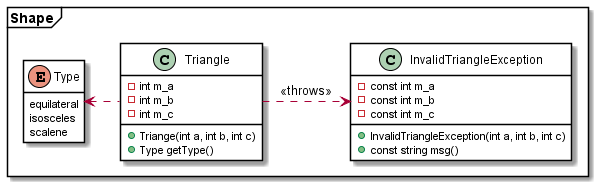
\includegraphics[scale=0.7]{figures/classdiagram.png}
    \caption{Statistic and FileUtil class UML}
    \label{fig:classdiagram}
\end{figure}


\newpage
\section{Source Code}
\begin{code}
\caption{Statistic.h}
\inputminted[breaklines, frame=single, linenos]{cpp}{code/Statistic.h}
\label{code:statistic.h}
\end{code}

\begin{code}
\caption{Statistic.cpp}
\inputminted[breaklines, frame=single, linenos]{cpp}{code/Statistic.cpp}
\label{code:statistic.cpp}
\end{code}

\begin{code}
\caption{FileUtil.h}
\inputminted[breaklines, frame=single, linenos]{cpp}{code/FileUtil.h}
\label{code:fileutil.h}
\end{code}

\begin{code}
\caption{FileUtil.cpp}
\inputminted[breaklines, frame=single, linenos]{cpp}{code/FileUtil.cpp}
\label{code:FileUtil.cpp}
\end{code}

\begin{code}
\caption{main.cpp}
\inputminted[breaklines, frame=single, linenos]{cpp}{code/main.cpp}
\label{code:main.cpp}
\end{code}


\newpage
\section{Test Driver}
\begin{code}
\caption{test.cpp}
\inputminted[breaklines, frame=single, linenos]{cpp}{code/test.cpp}
\label{code:test.cpp}
\end{code}

\section{Test Results}
\begin{figure}[H]
    \centering
    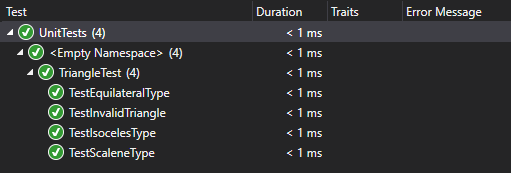
\includegraphics[scale=.8]{figures/TestResults.PNG}
    \caption{Test driver results}
    \label{fig:testresults}
\end{figure}

\end{document} 
